% -----------------------------*- LaTeX -*------------------------------
\documentclass[12pt]{report}
\usepackage{%
	amsfonts,%
	amsmath,%	
	amssymb,%
	amsthm,%
	algorithm,%
	babel,%
	bbm,%
	etex,%
	%biblatex,%
	caption,%
	centernot,%
	color,%
	dsfont,%
	enumerate,%
	epsfig,%
	epstopdf,%
	geometry,%
	graphicx,%
	hyperref,%
	latexsym,%
	mathtools,%
	multicol,%
	pgf,%
	pgfplots,%
	pgfplotstable,%
	pgfpages,%
	proof,%
	psfrag,%
	subfigure,%	
	tikz,%
	ulem,%
	url%
}	
\usepackage[noend]{algpseudocode}
\usepackage[mathscr]{eucal}
\usepgflibrary{shapes}
\usetikzlibrary{%
  	arrows,%
	backgrounds,%
	chains,%
	decorations.pathmorphing,% /pgf/decoration/random steps | erste Graphik
	decorations.text,%
	matrix,%
  	positioning,% wg. " of "
  	fit,%
	patterns,%
  	petri,%
	plotmarks,%
  	scopes,%
	shadows,%
  	shapes.misc,% wg. rounded rectangle
  	shapes.arrows,%
	shapes.callouts,%
  	shapes%
}

\theoremstyle{plain}
\newtheorem{thm}{Theorem}[section]
\newtheorem{lem}[thm]{Lemma}
\newtheorem{prop}[thm]{Proposition}
\newtheorem{cor}[thm]{Corollary}

\theoremstyle{definition}
\newtheorem{defn}[thm]{Definition}
\newtheorem{conj}[thm]{Conjecture}
\newtheorem{exmp}[thm]{Example}
\newtheorem{assum}[thm]{Assumptions}
\newtheorem{axiom}[thm]{Axiom}

\theoremstyle{remark}
\newtheorem{rem}{Remark}
\newtheorem{note}{Note}
\newtheorem{fact}{Fact}

\newcommand{\norm}[1]{\left\lVert#1\right\rVert}
\newcommand{\indep}{\!\perp\!\!\!\perp}
\DeclarePairedDelimiter\abs{\lvert}{\rvert}%
\newcommand\numberthis{\addtocounter{equation}{1}\tag{\theequation}}
\newcommand{\tr}{\operatorname{tr}}
\newcommand{\R}{\mathbb{R}}
\newcommand{\N}{\mathbb{N}}
\newcommand{\E}{\mathbb{E}}
\newcommand{\Z}{\mathbb{Z}}
\newcommand{\B}{\mathscr{B}}
\newcommand{\C}{\mathcal{C}}
\newcommand{\T}{\mathscr{T}}
\newcommand{\F}{\mathcal{F}}
\newcommand{\G}{\mathcal{G}}
%\newcommand{\ba}{\begin{align*}}
%\newcommand{\ea}{\end{align*}}
\DeclareMathOperator*{\argmax}{arg\,max}
\renewcommand{\qedsymbol}{$\blacksquare$}
\makeatletter
\def\BState{\State\hskip-\ALG@thistlm}
\makeatother

\makeatletter
\def\th@plain{%
  \thm@notefont{}% same as heading font
  \itshape % body font
}
\def\th@definition{%
  \thm@notefont{}% same as heading font
  \normalfont % body font
}
\makeatother
\date{}
\usepackage{graphicx}
\graphicspath{ {Figures/} }
\usepackage{scribe_e1244}
\usepackage{times}
%\newtheorem{defn}[thm]{Definition}
%\newtheorem{lem}{Lemma}[thm]
%\newenvironment{definition}[1][Definition]{\begin{trivlist}
%\item[\hskip \labelsep {\bfseries #1}]}{\end{trivlist}}
\begin{document}
\lecturer{Aditya Gopalan}		
\scribe{B Phanidhar \& Soumya Subhra Banerjee}	% required, put your name here
\lecturenumber{7}			% required, must be a number
\lecturedate{January 24}		% required, omit year
\maketitle

% title of the lecture
\begin{center}
{\Large \bf Composite Hypothesis Testing}
\end{center}


% ----------------------------------------------------------------------

\section{Recap of Composite Hypothesis Testing}

The simple hypothesis-testing problem is called so because each of the two hypothesis corresponds to only a single distribution for the observation.On the contrary,in a composite hypothesis-testing problem there may be several distributions corresponding to the same hypothesis.The number of hypotheses however remains same ,i.e two for binary hypothesis testing.Here, we shall restrict ourselves to two hypotheses and exclude discussions on $M$-ary hypothesis testing.
\\
\\ The chief components to define composite hypothesis testing are as follows:

\begin{itemize}
\item {\bf \em Parameter Space}: $\Lambda$ 
\item {\bf \em Observation Space}: $\Gamma$
\item {\bf \em Probability distributions}:  $\mathbbm{P}_\theta$ ,defined on $\Gamma,\forall$ $\theta \in \Lambda$ 
\\Note,$\Lambda$ can be a countable or an uncountable set.Broadly, some of the distributions pertaining to it's elements correspond to $H_0$ and some correspond to $H_1$.
\item {\bf \em Decision rule(non-randomized)}:  $\delta: \Gamma \to \{0, 1\}$
\item {\bf \em Costs}:  $C(i,\theta)$: Cost for declaring $H_i$ when the true distribution is $\mathbb{P}_{\theta}$\\$\forall$ i$\in$\{0,1\} ,$\forall \theta\in\Lambda$ .We can have different costs modelled on different values of $\theta$.
\item {\bf \em Conditional Risks}: for a decision rule $\delta$, is defined for any given $\theta$ as, 
\begin{align*}
\mathbb R_\theta(\delta)&\bydef\mathbb{E}_{\theta}[C(\delta(Y),\theta)]
\end{align*}
where $\mathbb{E}_{\theta}$ denotes expectation assuming $Y\sim \mathbb{P}_{\theta}$.
\item {\bf \em Bayes Risk}: The average conditional risk under a prior $\pi$ on $\Lambda$ , 
\begin{align*}
r(\delta)&\bydef\mathbb{E}[C(\delta(Y),\Theta)]\\
\Theta&\sim\pi  \text{ on }  \Lambda
\end{align*}
where $\mathbb{E}\text{[.]}$ denotes expectation assuming $\Theta \sim\pi  \text{ on }  \Lambda$.
\end{itemize}

%-----------------------------------------------------page-1-end

\begin{note}
$\mathbb{E}\text{[.]}$ denotes expectation in the experiment which has two sources of randomness,
\begin{enumerate}
\item $\Theta\sim\pi$ ,over $\Lambda$
\item $Y\sim\mathbb{P}_\theta$ ,over $\Gamma$
\end{enumerate}
This is in fact, a generalization of a simple hypothesis testing problem.
\end{note}

\section{Finding the Bayes rule}
The Bayes risk is given by,
\begin{align*}
r(\delta) &= \mathbb{E}[C(\delta(Y),\Theta)]\\
&= \mathbb{E}[\mathbb{E}[C(\delta(Y),\Theta)|Y]] \text{ (by iterated expectation)}\\
\end{align*}
Observe that if we fix $Y=y$, $\delta(y)$ can take values either 0 or 1.Hence, we can write $r(\delta)$ as follows,

\begin{equation}
r(\delta)={\Large \int_{\Gamma}}
\begin{cases}
\mathbb{E}[C(0,\Theta)|Y=y]p(y)dy, \text{  if } \delta(y)=0\\
\mathbb{E}[C(1,\Theta)|Y=y]p(y)dy, \text{  if } \delta(y)=1\\
\end{cases}
\end{equation}

\noindent To reduce $r(\delta)$ we choose $\delta(y)$ to take the minimum of the above expectations.\\
Since we have to design $\delta(y) \in$ \{0,1\} $\forall y \in \Gamma$, an optimal Bayes rule would be,

\begin{equation}
\delta(y)=
\begin{cases}
1, \text{ if }\mathbb{E}[C(1,\Theta)|Y=y]< \mathbb{E}[C(0,\Theta)|Y=y]\\
0, \text{ o.w.}\\
\end{cases}
\end{equation}

(Note: Breaking ties does not affect the Bayes risk.)\\
The above expectations are expected costs under the aposteriori distribution on $\Theta$ after observing $y$ , i.e., with no observation initial priors are used,the prior is updated with a posterior distribution on observing some $y$. 
\begin{rem}
A Bayes rule with prior $\pi$ on $\Theta$, and observation $y$ $\equiv$ A Bayes rule with prior : (posterior distribution of $\Theta|Y$), and observation $\phi$ (i.e., no observation)
\end{rem}

\subsection{Uniform cost (an important special case):}
{\em Uniform costs:}  Uniform costs over disjoint subsets of $\Lambda$ is defined as the following.
\begin{align*}
\Lambda = \Lambda_0 \cup \Lambda_1 , \Lambda_0 \cap \Lambda_1= \phi\\ 
\&,C(i,\theta)=C_{ij} \forall \theta \in \Lambda_j\\
\text{for } i,j \in \{0,1\}\\
\end{align*}

%=======================================================Page-2end
\noindent In other words,the uniform cost of declaring a hypothesis $H_i$ is same for all $\theta$ belonging to a disjoint subset of $\Lambda$.

\begin{figure}[h]
\centering
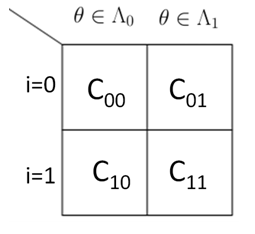
\includegraphics[scale=0.8]{Figures/UniCostComp.png}
\caption{Uniform Cost Table over two disjoint subsets for Composite Hypothesis Testing.}
\label{fig:uniformcost}
\end{figure}
\vskip .1cm
\noindent Assume $C_{11} < C_{01}$.
Thus,under uniform costs,

\begin{align*}
\mathbb{E}[C(0,\Theta)|Y=y]&\gtreqqless \mathbb{E}[C(1,\Theta)|Y=y]\\
\text{iff},~~
C_{00}\mathbb{P}[\Theta\in\Lambda_0|Y=y]+C_{01}\mathbb{P}[\Theta\in\Lambda_1|Y=y]&\gtreqqless C_{10}\mathbb{P}[\Theta\in\Lambda_0|Y=y]+C_{11}\mathbb{P}[\Theta\in\Lambda_1|Y=y]\\
\text{iff},~~\frac{\mathbb{P}[\Theta\in\Lambda_1|Y=y]}{\mathbb{P}[\Theta\in\Lambda_0|Y=y]}&\gtreqqless\frac{(C_{00}-C_{10})}{(C_{11}-C_{01})}\\
\text{iff},
~~\frac{\mathbb{P}[Y=y|\Theta\in\Lambda_1]\mathbb{P}[\Theta\in\Lambda_1]}
{\mathbb{P}[Y=y|\Theta\in\Lambda_0]\mathbb{P}[\Theta\in\Lambda_0]}&\gtreqqless\frac{(C_{00}-C_{10})}{(C_{11}-C_{01})}\text{,(by Bayes formula)}\\
\\
\text{iff},~~L(y)&\gtreqqless\tau\\
\text{where},~~L(y)&\bydef\frac{\mathbb{P}[Y=y|\Theta\in\Lambda_1]}
{\mathbb{P}[Y=y|\Theta\in\Lambda_0]},\\
\tau&\bydef \frac{\pi_0(C_{00}-C_{10})}{\pi_1(C_{11}-C_{01})},\\
\text{with},~~\pi_i&\bydef \mathbb{P}[\Theta\in\Lambda_i],i=0,1\\
\end{align*}


\begin{rem}
 With uniform costs over $\Lambda_0$ and $\Lambda_1$, the optimal Bayes rule is again a likelihood ratio test.\\
\end{rem}

%===================================================Page-3 end
\begin{rem}
We can write
\begin{align*}
\mathbb{P}[{Y=y}|{\Theta\in\Lambda_1}]=\int_{\Lambda} p_{\theta}(y)w_1({\theta})d\theta=\int_{\Lambda_1}p_{\theta}(y)w_1({\theta})d\theta\\
\text {where },~~w_1(\theta)=
\begin{cases}
0,~~~~~~~~\text{if}~ \theta\notin\Lambda_1\\
\frac{\pi(\theta)}{\int_{\Lambda_1} \pi({\theta^`})d\theta^`},~\text{if}~ \theta\in\Lambda_1\\
\end{cases}
\end{align*}

\begin{figure}[h]
\centering
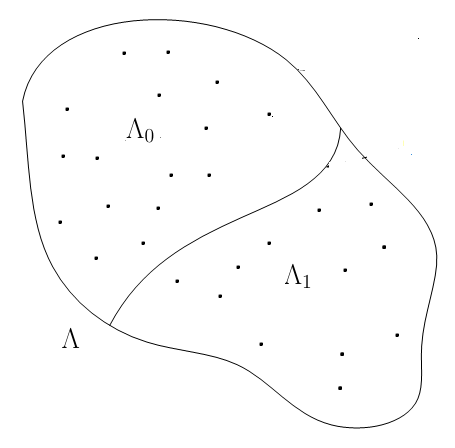
\includegraphics[scale=0.6]{Figures/Lambdaparameterspace.png}
\caption{The Parameter space $\Lambda$ and with distribution $\Theta\sim\pi$, over $\Lambda$.}
\label{fig:pionlambda}
\end{figure}

(\noindent $\pi$ puts a distribution (i.e., $\pi(\theta),\theta\in\Lambda$) over whole $\Lambda$.We can say, $w_1(\theta)$ is the scaled probability of what $\pi$ puts on a $\theta$ in $\Lambda_1$.)
\end{rem}

\begin{exmp}
{\em 2-D Location testing with Gaussian noise}\\

\begin{figure}[h]
\centering
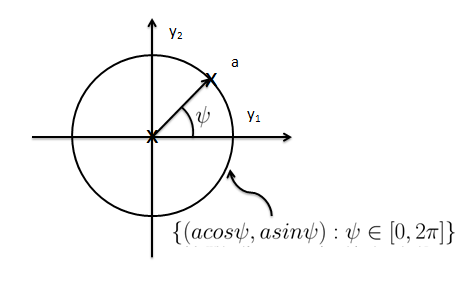
\includegraphics[scale=0.8]{Figures/2D-Gaussian-loctest.png}
\caption{Distributions of hypotheses in 2-D location testing with Gaussian noise.}
\label{fig:2dgaussloctest}
\end{figure}
\noindent Here the null hypothesis has a mean zero bi-variate Gaussian distribution which denotes pure noise (denoted by the origin in figure \ref{fig:2dgaussloctest}), while the alternate hypothesis has multiple bi-variate Gaussian distributions with mean lying on the circle of radius $a$.\\
\\
{\em Goal:}  Detect signal (point on circle) or no signal (origin) in Gaussian noise.\\
\begin{align*}
\Gamma = \mathbb{R}^2,[i.e.,Y=(Y_1,Y_2)^{T}],\sigma^2 \in \R_+, a \in \R_+,\\
\end{align*}
\begin{align*}
&H_0:Y\sim\mathcal{N}(\left(\begin{smallmatrix}0 \\ 0\end{smallmatrix}\right),\sigma^2 I)\\
&H_1:Y\sim\mathcal{N}(\left(\begin{smallmatrix}a\cos{\psi} \\ a\sin{\psi}\end{smallmatrix}\right),\sigma^2 I),\\
\text{with},&\Psi\sim unif[0,2\pi],
\end{align*}
%==========================================Page-4-end
This problem is called ``NON COHERENT DETECTION PROBLEM" in communication theory.\\
{\bf \em Parameter space:}\\
\begin{align*}
\Lambda &=\overbrace{\{0,a\}}^{``\theta_1"}\times\overbrace{[0,2\pi]}^{``\theta_2"}\\
\Lambda_0 &=\{\theta\in\Lambda : \theta_1=0\}\\
\Lambda_1 &=\{\theta\in\Lambda : \theta_1=a\}\\
\text{where},~~\theta&\equiv(\theta_1,\theta_2)\\
\end{align*}
Assume uniform costs over $\Lambda_0, \Lambda_1.$\\
(Note, $\theta_2$ pertains to $\psi$ in figure \ref{fig:2dgaussloctest}.Also, $\theta_1=0$,with any value of $\theta_2$, pertains to the point at origin.)\\
We can write,
\begin{equation}
L(y) ={\frac{P(y|\Theta \in \Lambda_1)}{P(y|\Theta\in \Lambda_0)}}\\\\
\end{equation}
Where,\\
{\em Denominator:}
\begin{align*}
P(y|\Theta \in \Lambda_0) = {\frac{\exp(\frac{-y^2_1-y^2_2}{2\sigma^2})}{2\pi\sigma^2}}\\
\end{align*}
{\em Numerator:}
\begin{align*}
P(y|\Theta \in \Lambda_1)={\frac{1}{2\pi}}{\int_{0}^{2\pi} \frac{\exp(\frac{-(y_1-a\cos\theta_2 )^2 -(y_2-a\sin\theta_2)^2}{2\sigma^2})}{2\pi\sigma^2}}d\theta_2\\
\text{(by averaging over $\theta_2\in[0,2\pi])$}\\
\end{align*}
hence,
\begin{equation}
L(y)={\frac{\exp(\frac{-a^2}{2\sigma^2})}{2\pi}}{\int_{0}^{2\pi}} {\exp(\frac{a(y_1\cos\theta_2+y_2\sin\theta_2)}{\sigma^2})d\theta_2}\\
\end{equation}
Changing to polar co-ordinates,
\begin{align*}
r \bydef \sqrt(y_1^2+y_2^2)\\
\phi \bydef \arctan(\frac{y_2}{y_1})
\end{align*}
We get $L(y)$ as follows,
\begin{align*}
L(y)&= {\frac{\exp(\frac{-a^2}{2\sigma^2})}{2\pi}}{\int_{0}^{2\pi}} {\exp({\frac{ar\cos(\theta_2-\phi)}{\sigma^2}})d\theta_2}\\        
      &= {\frac{\exp(\frac{-a^2}{2\sigma^2})}{2\pi}}{\int_{0}^{2\pi}} {\exp({\frac{ar\cos{u}}{\sigma^2}})du}~~\text{,where $u=\theta_2-\phi$.}\\
      &= {\exp({\frac{-a^2}{2\sigma^2}})}.I_0({\frac{ar}{\sigma^2}})\\
\end{align*}
Here$\ I_0{(x)}$ is the modified Bessel function,given by,\\
\begin{align*}
I_0(x) \bydef {\frac{1}{2\pi}} {\int_{0}^{2\pi}} {\exp(x\cos{u})du}\\
\end{align*}
\begin{figure}[h]
\centering
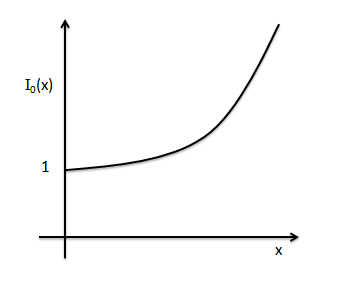
\includegraphics[scale=0.8]{Figures/modifiedbessel.png}
\caption{The modified Bessel function.}
\label{fig:modbessl}
\end{figure}
Note that $L(y)$ does not depend on $\theta_2$ in the final expression.Hence,
\begin{align*}
L(\left(\begin{smallmatrix}y_1 \\ y_2\end{smallmatrix}\right)) &\gtreqqless \tau \\ 
\Leftrightarrow r=\sqrt(y_1^2+y_2^2)  &\gtreqqless I_0^{-1}(\tau \exp(\frac{a^2}{2\sigma^2})) {\frac{\sigma^2}{a}} \\
\end{align*}
\end{exmp}

\end{document}

